%% Template for ENG 401 reports
%% by Robin Turner
%% Adapted from the IEEE peer review template

%
% note that the "draftcls" or "draftclsnofoot", not "draft", option
% should be used if it is desired that the figures are to be displayed in
% draft mode.

\documentclass[peerreview]{IEEEtran}
\usepackage{url} % Provides better formatting of URLs.
\usepackage[utf8]{inputenc} % Allows Turkish characters.
\usepackage[style=ieee,sortcites=true,sorting=nyt,backend=biber]{biblatex}
\usepackage{booktabs} % Allows the use of \toprule, \midrule and \bottomrule in tables for horizontal lines
\usepackage{graphicx}
\usepackage{amsmath}
\usepackage{amssymb}
\addbibresource{bibliography.bib}

\begin{document}
%\begin{titlepage}
% paper title
% can use linebreaks \\ within to get better formatting as desired
\title{Evaluating the Capability of Pix2Pix in Producing Synthetic Images}


% author names and affiliations

\author{Arsyi Syarief Aziz \\ Muh. Yusuf Syam \\ Aso Ahmad Amin Rais \\
Computer Science Study Program\\
Universitas Hasanuddin\\
}
\date{22/6/22}

% make the title area
\maketitle
\tableofcontents
\listoffigures
\listoftables
%\end{titlepage}

\IEEEpeerreviewmaketitle
\begin{abstract}
Pix2Pix is a general purpose framework that is designed for image-to-image translation. This framework implements the conditional type of the generative adversarial network, known as the cGAN. The use of cGANs in this framework allows it to be used in various context, such as image reconstruction, and image coloring. To explore this capability, we have conducted an evaluation on the framework to test its ability in imitating images from three different datasets: \textit{maps}, \textit{edges2shoes}, and \textit{facades}. The assessment of the framework's performance was done by manual inspection though the use of a quick response program. The result of this evaluation shows that Pix2Pix was able to successfully synthesize realistic looking images for two of the three datasets.

\end{abstract}

\section{Introduction}
In this technical report, we will discuss about the capability of the Pix2Pix framework in synthesizing realistic images.

Pix2Pix in this report is defined as a general purpose framework that is designed for image-to-image translation. This framework is built upon the idea of a generative adversarial network (GAN), specifically the conditional type. The use of conditional GANs in this context allows the network to generate image samples that correspond to a given label image. 

Many people have demonstrated the use of this framework to generate images in many context, such as image reconstruction, image coloring. To further explore the flexibility of this framework, we will evaluate its capability in imitating images from three different datasets: \textit{maps}, \textit{edges2shoes}, and \textit{facades}. 

More details about the framework and our evaluation methodology are explained in the following sections.

\section{Problem Defintion}
This technical report focuses on understanding the capability of the Pix2Pix framework in synthesizing realistic looking images. To understand this capability, we have completed a few experiments on the framework, testing it on three different datasets from \cite{berkeley2017}. Ultimately, through the results of these experiments we will answer one important question regarding the Pix2Pix framework: Is it able to produce realistic looking images for different types of images?

\section{Related Works}
Before we explain about the Pix2Pix framework, we will first explain about the underlying concepts that construct it. Specifically speaking, this section will provide the definition of the generative adversarial network and the conditional generative adversarial network.

\subsection{Generative Adversarial Network}
Generative adversarial network (GANs) were created by \cite{goodfellow2014generative} to provide a framework to estimate generative models. It works though an adversarial process where two model compete with each other to be better than their counterpart. These models are a generator $G$, used to capture a data distribution, and a discriminator $D$, used to predict whether a sample is synthetic or not.

The training process of this framework consists of three steps. First, the generator generates a synthetic image from a random distribution $p_z(z)$. Second, the generated synthetic image is inputted into the discriminator along with a real image, where the discriminator is tasked to correctly identify the synthetic image. Third, the parameters of the two models are updated based on the results of the prediction. This process is repeated continuously until the generator is able to consistently fool the discriminator.

The above explanation might seem intuitive as it is analogous to how a criminal would learn to create counterfeit money and avoid law enforcement, however it is just a simplification of what actually occurs during training. To formally define the training process, we state the following goals of the models. For the generator model, its goal is to learn a function $G(z;\theta_g$) such that it maps a random noise $p_z(z)$ to the data space. Meanwhile, for the discriminator, its goal is to learn a function $D(x;\theta_d$) that outputs a scalar value that represents the probability that an input $x$ originates from training data and not from the generator \cite{goodfellow2014generative}. 

In addition to generating images by the use of a generator and identifying images through a discriminator, we have also previously stated that the parameters of the models have to be updated based on the results of the prediction. These parameters follow a formula. For the generator, its parameters are updated to minimize $\log{(1-D(G(z)))}$, and for the discriminator, parameters are updated to maximize $\log{(D(x))}$. 

As one might be able to see, the described training process of a GAN follows the minimax game \cite{goodfellow2014generative}. Thus, by defining V(D, G) as its value function, we can define the objective function as equation \ref{eq:GAN}.

\begin{equation} \label{eq:GAN}
\begin{split}
\min_{G} \max_{D} V(D, G) = & \mathbb{E}_{x \sim p_{data}(x)} \left[ \log{D(x)} \right] + \\
&\mathbb{E}_{z\sim p_z{z}}\left[ \log{(1-D(G(z)))}\right]
\end{split}
\end{equation}

\begin{figure}[t]
\centering
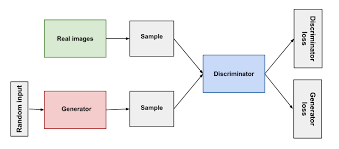
\includegraphics[width=0.8\columnwidth]{GAN.png} 
\caption{Structure of the GAN framework \cite{googledevelopers2019ganstructureimage}}.
\label{fig:GAN}
\end{figure}

\subsection{Conditional Generative Adversarial Networks}
Conditional generative adversarial networks (cGANs) are a variant of GANs that condition the generator and disciminator based on some information $y$ \cite{mirza2014conditional}. This conditioning allows cGANs to be able to produce samples that correspond to $y$, such as samples that belong to a specific class.

Implementation wise, cGANs are similar to normal GANs, however, as we have stated, its models are conditioned on $y$. To condition these models, we add $y$ to both of their inputs. For the generator, we use $y$ and some random noise vector $z$ and map them to the data space, and for the discriminator we use $y$ and input data $x$ to identify whether $x$ originates from training data or from the generator. 

From this description, we can define the objective function of cGANs as equation \ref{eq:cGAN}.

\begin{equation}\label{eq:cGAN}
\begin{split}
\min_{G} \max_{D} V(D, G) = & \mathbb{E}_{x \sim p_{data}(x)} \left[ \log{D(x|y)} \right] + \\
&\mathbb{E}_{z\sim p_z{z}}\left[ \log{(1-D(G(z|y)))}\right]
\end{split}
\end{equation}

\begin{figure}[t]
\centering
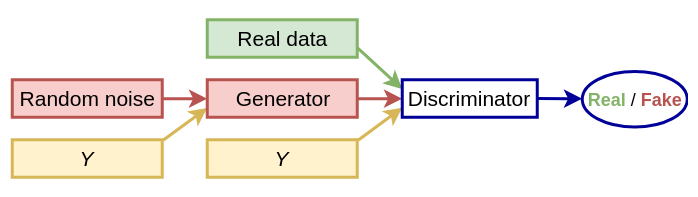
\includegraphics[width=0.8\columnwidth]{cGAN.png} 
\caption{Structure of the cGAN framework \cite{nayak2019cganimage}}.
\label{fig:cGAN}
\end{figure}

\section{Pix2Pix}
Pix2Pix was created by \cite{isola2017image} to provide a common framework to conduct picture-to-picture translation. More specifically speaking, it is used to translate a representation image of an object, called a label image, to a synthetic image that resembles an object. 

The following subsections will explain about the Pix2Pix framework though the description of its objective function, network architecture, and how it is optimized.  

\subsection{Objective Function}
Pix2Pix is built upon the cGAN framework. In this implementation, a label image is used to condition both the generator and discriminator to generate images corresponding to that label image. In addition to using cGANs, Pix2Pix also implements the L1 distance in its objective function. This addition helps helps Pix2Pix capture low frequencies \cite{isola2017image}.

From this description, we can define the objective function of the Pix2Pix framework 

\begin{equation}\label{eq:Pix2Pix}
G^{*} = \arg \min_{G} \max_{D} \mathcal{L}_{cGAN}(G, D) + \lambda\mathcal{L}_{L1}(G).
\end{equation}

\subsection{Model Architecture}
Pix2Pix implements two different architectures for its generator and discriminator. For its generator, Pix2Pix implements the "U-Net" architecture. Meanwhile, for its discriminator, Pix2Pix implements the "PatchGAN" architecture.

\subsubsection{U-Net}
U-Net is an implementation of the encoder-decoder architecture that contains skip connections in between its encoder and decoder blocks. The addition of these skip connections allow the U-Net architecture to avoid data bottlenecks which are caused by the downsampling and upsampling processes. Additionally, it also allows low level information from the input image to be easily propagated to the resulting output image \cite{isola2017image}.

The U-Net architecture consists of two main parts, which are:

\begin{itemize}
    \item \emph{The contracting path} (left of Fig.\ref{fig:U-Net}) which is built by a general convolutional process that downsamples sample data during information extraction.
    \item \emph{The expansive path} (right of Fig.\ref{fig:U-Net}) which is built by transposed 2D convolutional layers that upsamples information. 
\end{itemize}

%Gambar diinput di awal jaringan (kiri-atas). Data tersebut kemudian disebarkan melalui semua jalur yang mungkin dan, pada akhirnya, segmentation map keluar.

\begin{figure}[t]
\centering
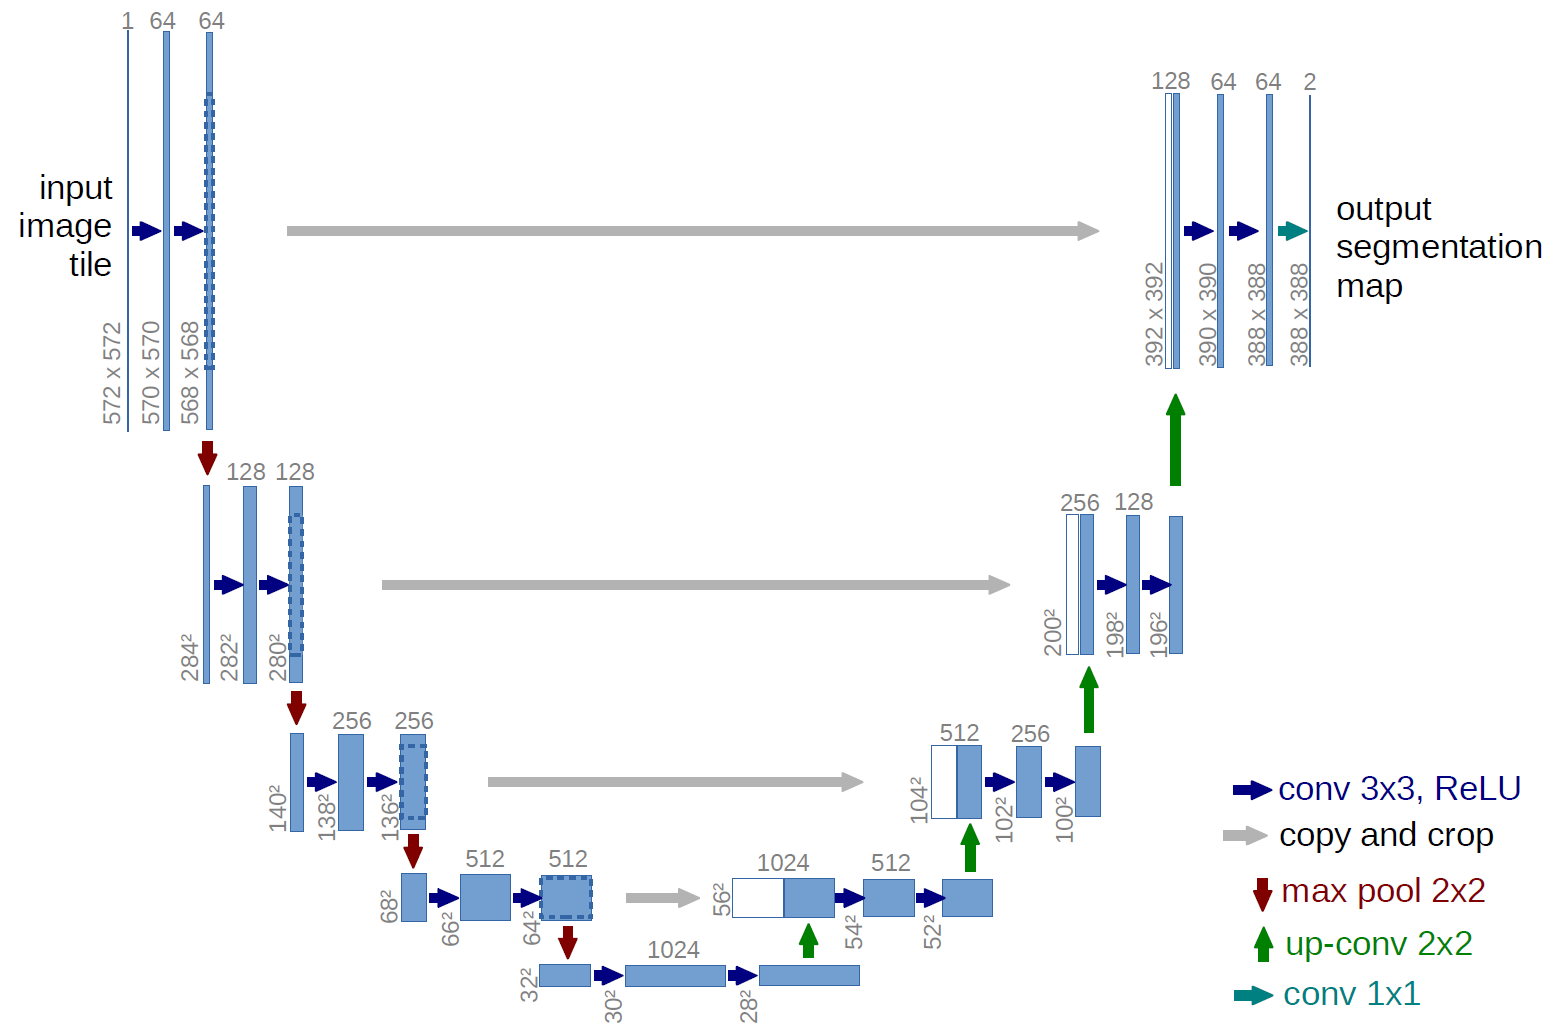
\includegraphics[width=0.8\columnwidth]{u-net-architecture.png} 
\caption{U-Net architecture \cite{olaf2015unetimage}}
\label{fig:U-Net}
\end{figure}

\subsubsection{PatchGAN}
PatchGAN, also known as the Markovian discriminator is a type of discriminator that classifies an image by dividing the image into blocks of size $NxN$, known as patches.

To classify the images, the discriminator does a convolution on all the patches in an image and tries to classify whether or not the patches represent real or fake images. The result of each of these classifications is not a scalar, but an array of size $NxN$, where each element of the array has a value in the range of [0-1]. The result of the overall classification of the image is obtained by finding the average value of each patch.

Dividing an image into several patches is advantageous to the models performance. By reducing the image into small patches, then the number of parameters required by the model is thus reduced (see \cite{isola2017image}).

%Membagi citra menjadi beberapa patch menguntungkan dari segi performa, karena semakin kecil ukuran patch, maka parameter yang dimiliki oleh GAN akan lebih sedikit.

\subsection{Optimization}
Optimization of the networks in this framework follows the standard approach from \cite{goodfellow2014generative}. In this approach, we alternate between one gradient descent step on $D$ and one gradient decent step on $G$. However, rather than training $G$ to miniminize $\log (1-D(x, G(x,z))$, this framework instead trains to maximize $\log D(x, G(x, z))$ \cite{isola2017image}. Additionally, we also divide the objective function by 2 when optimizing $D$, which helps slow down the learning rate of $D$ relative to $G$.

\section{Criteria for Assessing the Framework}
The criteria we used to assess the Pix2Pix framework is based on whether or not it is capable of producing realistic looking images. As it can be difficult to define a quantitative measure for this criteria, we conducted this assessment based on manual inspection of the images through the use of a quick response program.

This program evaluates 50 random images relating to a specific data set, which include 25 real images (the control group) and 25 fake images (the experimental group). Each of these images are displayed one-by-one and at random to an human assessor, who is given a few seconds to identify whether or not the corresponding image is real or fake. After assessing all the images, the program will display the number of correct identifications for both the control group and the experimental group, as well as the label image, ground truth image, and predicted image corresponding to the each of the random images.

\section{Methodology}
To provide an understanding of how our experiments were conducted, this section will explain about the methodology of our experiments. This includes an explanation about the datasets and the hyperparameters used. 

\subsection{Dataset}
The datasets we used in our experiments are three of the datasets used in the original Pix2Pix paper, which include the \textit{facades}, \textit{maps}, and \textit{edges2shoes} data sets. These datasets can be retrieved from \cite{berkeley2017}.

Each of these data sets consists of ground truth image and label image pairs. Firstly, in the facades dataset, the ground truth images are pictures of building facades and its label images are architectural elements the buildings. Secondly, in the maps data set, its ground truth images are satellite photos and its label images are map images. Finally, in the edges2shoes data set, the ground truth images are pictures of shoes and its label images are sketches of shoes.

\subsection{Hyperparameters}
For each of the data sets, we trained a separate Pix2Pix model which use the same hyper-parameters. These hyper-parameters include the use of mini-batch SGD and the Adam optimizer with a learning rate of 0.0002 and a $\beta_1$ value of 0.5, as well  as a total of 100 epochs.

\section{Analysis and Interpretation}
Table \ref{tab:results} shows the results of our evaluation. In this table, we can see that for both the \textit{maps} and \textit{edges2shoes} datasets, our human assessor was only able to correctly identify 60\% of the synthetic images and 72\% of the real images. This indicates that the models were able to synthesize a few realistic images for these data sets. However, it also indicates that our human assessor had some difficulty in identifying the real images, which can be attributed to the low resolution of the images (see fig \ref{fig:mapsrealincorrect} and fig \ref{fig:edges2shoesrealincorrect}). For the \textit{facades} dataset, our human assessor was able to identify almost all of the images correctly (96\% of real images and 96\% of fake images). This indicates that our Pix2Pix model could not produce realistic looking images for this dataset. 

Upon close inspection of the resulting images (see Appendix), we made a couple of discoveries related to Pix2Pix's ability in producing realistic images. The first discovery was that Pix2Pix favors simple label images, such as the edges used in the edges2shoes dataset. The second discovery was that Pix2Pix favors label images that preserves a lot of information from its ground truth image. This idea is supported by the fact that the edges2shoes and the maps datasets (which contain label images that are just a simplification of the ground truth images) were able to be used to synthesize a few realistic images. Meanwhile, the facades dataset (which contain label images that are only architectural elements of a building) had difficulty producing elements not shown by the label image, such as the roof of buildings.

\begin{figure}[t]
\centering
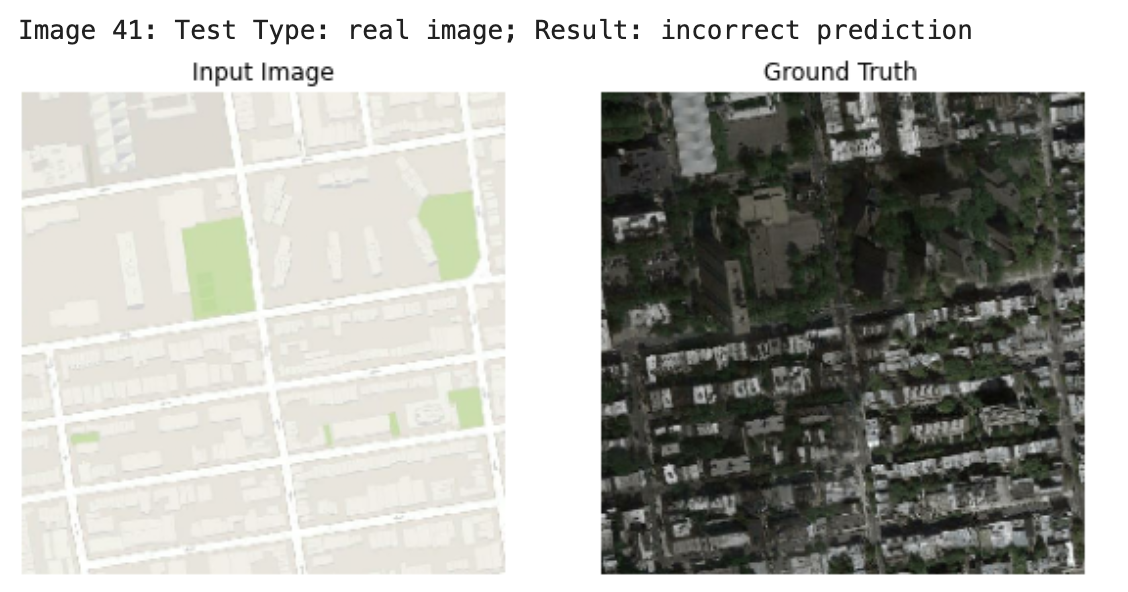
\includegraphics[width=0.8\columnwidth]{Maps real incorrect.png} 
\caption{A real \textit{maps} image which was incorrectly identified}.
\label{fig:mapsrealincorrect}
\end{figure}

\begin{figure}[t]
\centering
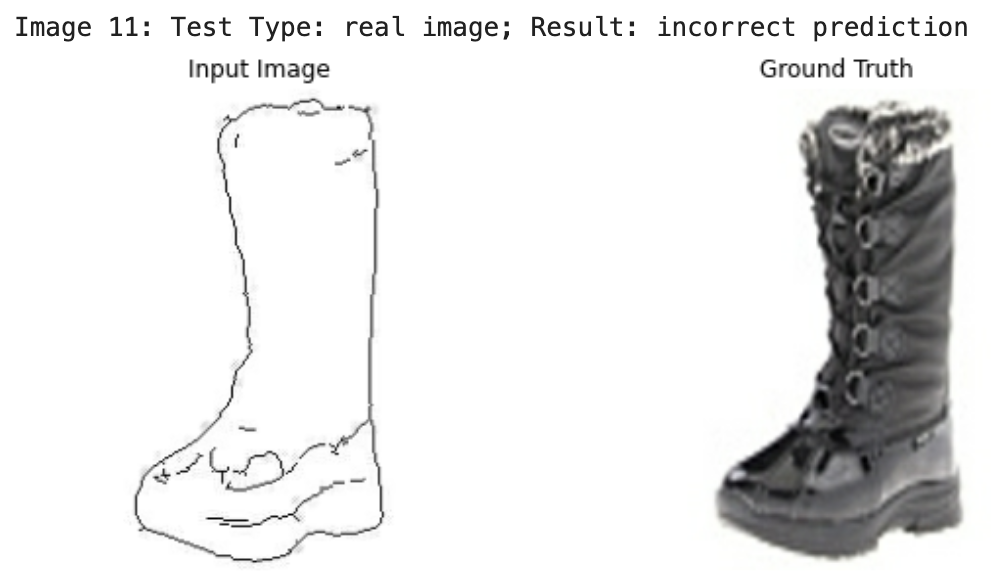
\includegraphics[width=0.8\columnwidth]{Edges2Shoes real incorrect.png}
\caption{A real \textit{edges2shoes} image which was incorrectly identified}.
\label{fig:edges2shoesrealincorrect}
\end{figure}


\begin{table}
\centering % Centers the table on the page, comment out to left-justify
\begin{tabular}{l c c} % The final bracket specifies the number of columns in the table along with left and right borders which are specified using vertical bars (|); each column can be left, right or center-justified using l, r or c. To specify a precise width, use p{width}, e.g. p{5cm}
\toprule % Top horizontal line
& \multicolumn{2}{c}{Group} \\ % Amalgamating several columns into one cell is done using the \multicolumn command as seen on this line
\cmidrule(l){2-3} % Horizontal line spanning less than the full width of the table - you can add (r) or (l) just before the opening curly bracket to shorten the rule on the left or right side
Dataset & Control (Real Image) & Experiment (Synthetic Image)\\ % Column names row
\midrule % In-table horizontal line
maps & 72\% & 60\% \\
edges2shoes & 72\% & 60\% \\
facades & 96\% & 96\% \\
\bottomrule % Bottom horizontal line
\end{tabular}
\smallskip 
\caption{Percentage of correctly identified images for each dataset}
\label{tab:results} 
\end{table}

\section{Conclusion and Recommendations}
The results of this technical report suggest that the Pix2Pix framework is able to synthesize realistic looking images for certain types of datasets. Out of the three datasets that we used, only two of them were able to successfully synthesize a reasonable amount of realistic images, these were \textit{maps} and \textit{edges2shoes} datasets. 

Following this conclusion, we recommend that further evaluation should be conducted on this framework with different datasets to better understand the capabilities of this framework.

\printbibliography


\appendices
\section{Image Samples} 
\begin{figure}[ht]
\centering
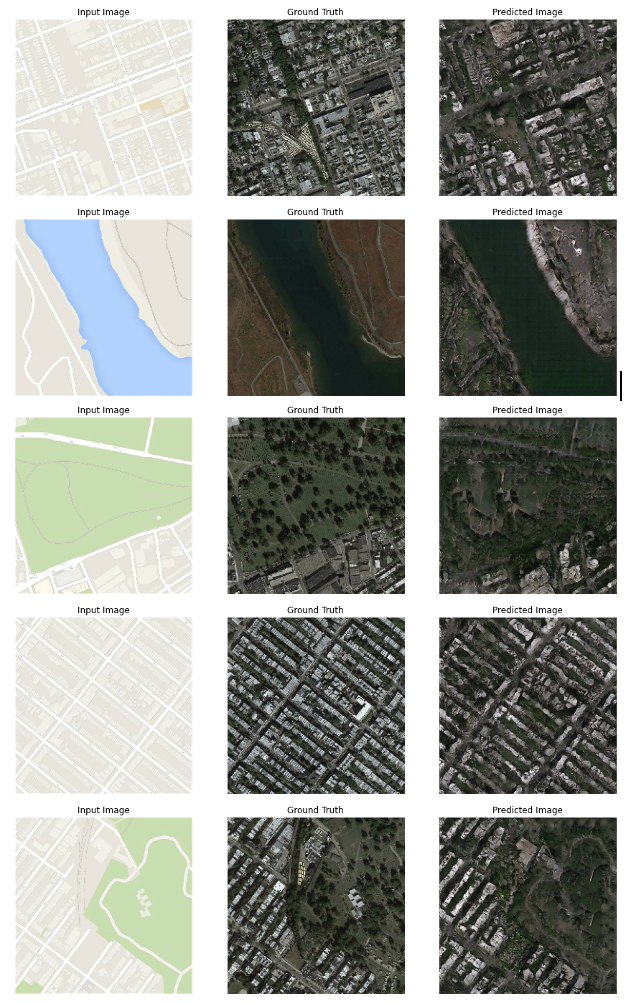
\includegraphics[width=0.6\columnwidth]{ex_maps.png} 
\caption{Five samples taken from the \textit{maps} dataset.}
\label{fig:ex_maps}
\end{figure}

\begin{figure}[ht]
\centering
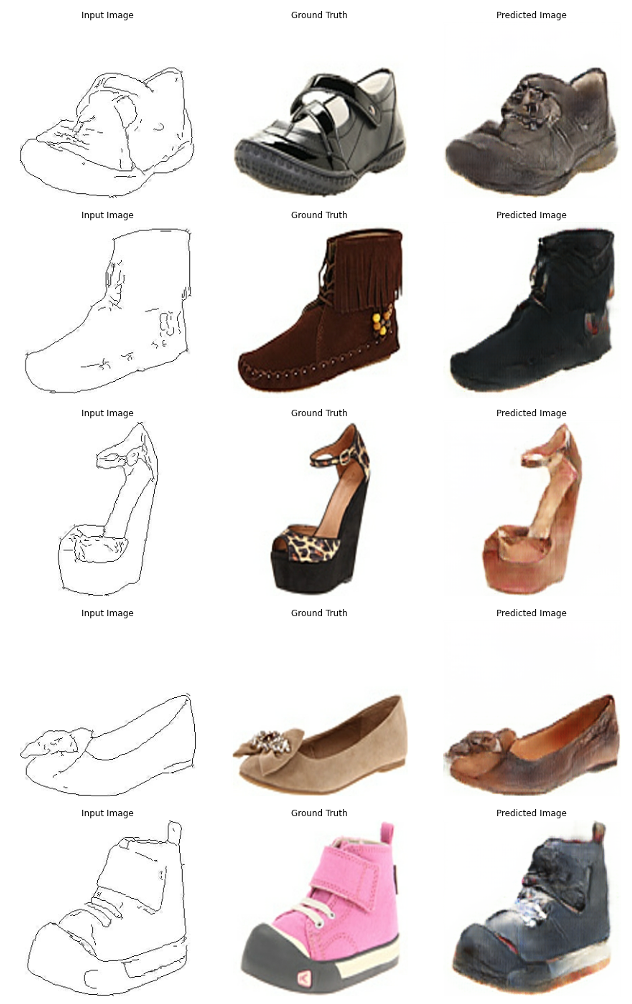
\includegraphics[width=0.6\columnwidth]{ex_edges2shoes.png} 
\caption{Five samples taken from the \textit{edges2shoes} dataset.}
\label{fig:ex_edges2shoes}
\end{figure}

\begin{figure}[!t]
\centering
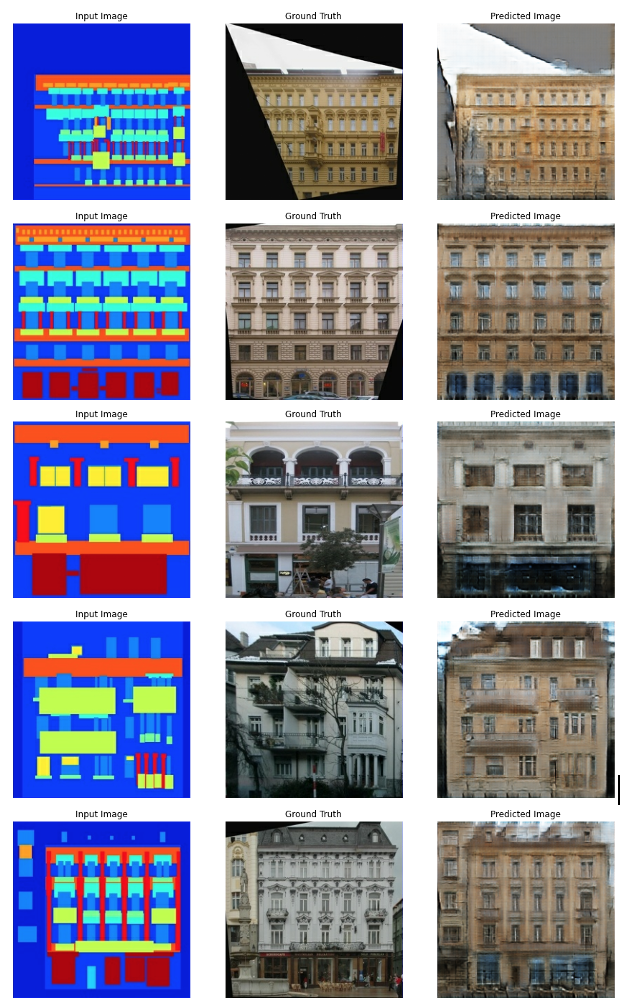
\includegraphics[width=0.6\columnwidth]{ex_facades.png} 
\caption{Five samples taken from the \textit{facades} dataset.}.
\label{fig:ex_facades}
\end{figure}




% This is a hand-made bibliography. If you want to use a BibTeX file, you're on your own ;-)














\end{document}


